\section{散射的形式理论}

考虑不含时的量子力学问题

\begin{equation}
H = H_0 + V
\end{equation}

假设$H_0$是自由的运动,

\begin{equation}
H_0 = \frac{p^2}{2m}
\end{equation}

其解记为

\begin{equation}
H_0 \left| \phi \right\rangle = E \left| \phi \right\rangle
\end{equation}

$H_0$对应的是入射粒子距离散射中心很远,或粒子被散射改变运动方向后又飞到距离散射中心很远的情形。两种情况$V$都可忽略不计。$H_0$的解可以是单色平面波\index{plane wave:平面波}(plane wave, $\left| p' \right\rangle$)或球面波\index{spherical wave:球面波}(spherical wave, $\left| klm \right\rangle$)。

在球坐标系下,我们可以证明

\begin{equation}
H_0 = - \frac{\hbar^2}{ 2m }  \frac{1}{r^2} \frac{\partial }{\partial r} r^2 \frac{\partial }{\partial r}  + \frac{L^2}{ 2m r^2}
\end{equation}

这里$L^2$是角动量算符的平方。本证函数可以按$R_{El} Y_{lm}$的方式分离变量,矢径部分:

\begin{equation}
- \frac{\hbar^2}{ 2m } \left( \frac{1}{r^2} \frac{\partial }{\partial r} r^2 \frac{\partial }{\partial r} - \frac{l (l + 1)}{ r^2}  \right) R_{El} = E R_{El}
\end{equation}

以上微分方程在变量变换

\begin{equation}
R_{El} = \frac{\chi_{El}}{r}
\end{equation}

下大大简化:

\begin{equation}
\chi'' + \left( \frac{2mE}{\hbar^2} - \frac{l(l+1)}{r^2} \right) \chi = 0
\end{equation}

当散射粒子远离散射中心时,$\frac{l(l+1)}{r^2}$项可忽略不计,同时考虑$E = \hbar^2 k^2 /2m$,微分方程变为:

\begin{equation}
\chi'' + k^2 \chi = 0
\end{equation}

它的解为:$e^{\pm i kr}$,再考虑到$R = \chi / r$,矢径部分的波函数为:

\begin{equation}
R_{El} (r) = \frac{e^{\pm i kr} }{r}
\end{equation}

我们可以把散射想象为三个区域:(1)粒子由无穷远入射,假设在$\hat z$方向上,波函数$\sim e^{i kz}$。(2)粒子在散射中心附近,$V$必须考虑,$H = H_0 +V $的本征值问题我们下面会展开讨论。(3)粒子被散射到无穷远去,如果只考虑弹性散射的话,波矢$k$的方向会改变,但大小不会变,此时哈密顿量为$H_0$,波函数$\sim \frac{e^{ikr}}{r} f( \theta, \phi )$。这里$\theta $和$\phi$是用来表示入射的$k \hat z$与散射的$k$的交角\footnote{在本笔记中我尽量不使用矢量的记号,主要目的是为了使公式看起来更简洁,如果你懂的话,自然会知道哪个字母表示的是矢量,哪个不是。}。

\subsection{李普曼-施温格方程}

假设散射是弹性的,$H_0 + V$也具有连续的能谱,并且本征值问题

\begin{equation}
( H_0 + V ) \left| \psi \right\rangle = E \left| \psi \right\rangle
\end{equation}

对应的E和$H_0 \left| \phi \right\rangle = E \left| \phi \right\rangle$对应的E是一样的。当$V \to 0$时,$\left| \psi \right\rangle \to \left| \phi \right\rangle$。

在形式上我们把$\left| \psi \right\rangle$记为:

\begin{equation}
\left| \psi \right\rangle = \frac{1}{E - H_0} V \left| \psi \right\rangle + \left| \phi \right\rangle
\end{equation}

对上式而言,(1)满足$V \to 0$,$\left| \psi \right\rangle \to \left| \phi \right\rangle$。(2)对$V \neq 0$,

\begin{equation}
(E - H_0 - V) \left| \psi \right\rangle = ( E - H_0 ) \left| \phi \right\rangle
\end{equation}

即

\begin{equation}
( E - H_0 ) \left| \psi \right\rangle = V \left| \psi \right\rangle + ( E - H_0 ) \left| \phi \right\rangle
\end{equation}

等式左右都左乘$( E - H_0)^{-1} $

\begin{equation}
\left| \psi \right\rangle = ( E - H_0)^{-1} V \left| \psi \right\rangle + \left| \phi \right\rangle
\end{equation}

为了保证算符$( E - H_0)^{-1} $有意义,将其改写为$\frac{1}{E - H_0 \pm i \epsilon}$,对应把$E$的定义由实数轴延拓到复数域上。

\begin{equation}
\left| \psi^{(\pm)} \right\rangle = \left| \phi \right\rangle + \frac{1}{E - H_0 \pm i \epsilon } V \left| \psi^{(\pm)} \right\rangle
\end{equation}

上式即所谓“李普曼-施温格方程”\index{Lippmann-Schwinger equation:李普曼-施温格方程}(Lippmann-Schwinger equation)。$\left| \psi^{(\pm)} \right\rangle$和“$\pm i \epsilon$”对应。

位置表象,

\begin{equation}
\left\langle x | \psi^{(\pm)} \right\rangle = \left\langle x | \phi \right\rangle + \int d^3 x' \left\langle x \right| \frac{1}{E- H_0 \pm i \epsilon} \left| x' \right\rangle \left\langle x' \right| V \left| \psi^{(\pm)} \right\rangle   
\end{equation}

对上式,定义积分的“核”是,

\begin{equation}
G_{\pm} (x, x') = \frac{\hbar^2}{2m} \left\langle x \right| \frac{1}{E- H_0 \pm i \epsilon} \left| x' \right\rangle
\end{equation}

可以证明:

\begin{equation}
G_{\pm} (x, x') = - \frac{1}{4 \pi} \frac{e^{\pm i k |x - x'|}}{|x - x'|}
\end{equation}

考虑$\left| \phi \right\rangle$是单色平面波,首先换到动量表象,

\begin{equation}
\left\langle x \right| \frac{1}{...}  \left| x' \right\rangle = \frac{\hbar^2}{2m} \int d^3 p' \int d^3 p'' \left\langle x | p' \right\rangle \left\langle p' \right| \frac{1}{E - \frac{p'^2 }{2m } \pm i \epsilon} \left| p'' \right\rangle \left\langle p'' | x' \right\rangle
\end{equation}

其中

\begin{equation}
\left\langle p' \right| \frac{1}{E - \frac{p'^2 }{2m } \pm i \epsilon} \left| p'' \right\rangle = \frac{ \delta^3 (p' - p'')  }{E - \frac{p'^2 }{2m } \pm i \epsilon}
\end{equation}

考虑单色平面波的表达式

\begin{equation}
\left\langle x | p' \right\rangle = \frac{e^{i p' \cdot x / \hbar }}{ (2 \pi \hbar)^{3/2}}
\end{equation}

现在积分变为

\begin{equation}
\frac{\hbar^2}{2m } \int \frac{d^3 p'}{( 2 \pi \hbar)^3} \frac{e^{i p' \cdot (x- x') / \hbar}}{E - \frac{p'^2 }{2m } \pm i \epsilon}
\end{equation}

选向量$x - x'$方向为极轴方向建立球坐标系,令$p' = \hbar q$,波矢$q$方向与$x - x'$方向的夹角为倾角$\theta$。$d^3 p' = \hbar^3 d^3 q = \hbar^3 q^2 dq \sin \theta d \theta d \phi $。积分限:

\begin{eqnarray*}
q & : & 0 \to \infty \\
\theta & : & 0 \to \pi \\
\phi & : & 0 \to 2 \pi
\end{eqnarray*}

变量变换:$\sin \theta d \theta = - d \cos \theta$, $ t = \cos \theta$

\begin{equation}
\frac{1}{(2 \pi)^3} \int_0^{\infty} q^2 dq \int_0^{2 \pi} d \phi \int_{-1}^1 \frac{d t  e^{i q |x - x'| t}}{k^2 - q^2 \pm i \epsilon} 
\end{equation}

这里假设$E = \frac{\hbar^2 k^2}{ 2m }$

\begin{eqnarray*}
I & = & \frac{1}{4 \pi^2}  \frac{1}{i | x-x' |} \int_0^{\infty} q dq \frac{ e^{i q |x-x'|} - e^{ - i q |x-x'|} }{k^2 - q^2 \pm i \epsilon }  \\
{} & = &  \frac{-1}{4 \pi^2} \frac{1}{i | x-x' |} \int_0^{\infty} q dq \frac{ e^{i q |x-x'|  }  - e^{-i q |x-x'|} }{ q^2 - k^2  \mp i \epsilon }  \\
{} & = & \frac{i}{4 \pi^2 | x-x' | }  \int_{- \infty}^{\infty} \frac{q dq e^{i q |x - x'|}}{ q^2 - k^2 \mp i \epsilon }
\end{eqnarray*}

考虑

\begin{equation}
\frac{1}{q - k \mp i\epsilon' } + \frac{1}{q + k \pm i \epsilon' } = \frac{2 q}{q^2 - k^2 \mp i \epsilon }
\end{equation}

\begin{figure}[htbp]
\begin{center}
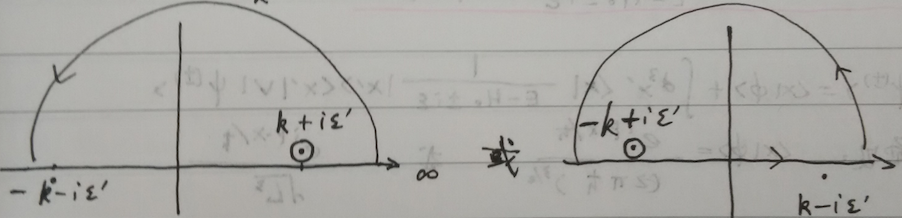
\includegraphics[width=10cm]{Scattering/TheContour.png}
\caption{奇点位置和积分回路。}
%\label{default}
\end{center}
\end{figure}


对“upper sign”,奇点位置:

\begin{equation}
q = k + i \epsilon' , q= - k - i \epsilon' 
\end{equation}

对“lower sign”,奇点位置:

\begin{equation}
q = k - i \epsilon' , q= - k + i \epsilon' 
\end{equation}

由于被积函数中出现的是$e^{i q |x - x'|}$,积分回路选上半回路(即$q: - \infty \to \infty$,然后上半回路绕回$q \to - \infty$)。对“upper sign”,回路绕过奇点:$q = k + i \epsilon'$,对“lower sign”,回路绕过奇点:$q= - k + i \epsilon'$。

根据留数定理\index{Residue theorem:留数定理}:

\begin{equation}
I = \frac{i}{4 \pi^2 }\frac{2 \pi i}{2} \frac{e^{ \pm i k |x-x'|}}{|x-x'|}  = - \frac{1}{4 \pi} \frac{e^{ \pm i k |x-x'|}}{|x-x'|}
\end{equation}

即

\begin{equation}
G_{\pm} (x, x') = - \frac{1}{4 \pi} \frac{e^{\pm i k |x - x'|}}{|x - x'|}
\end{equation}

因此

\begin{equation}
\left\langle x | \psi^{(\pm)} \right\rangle = \left\langle x | \phi \right\rangle - \frac{2m}{\hbar^2} \int d^3 x' \frac{e^{\pm i k |x-x'|}}{4 \pi |x-x'| } \left\langle x' \right| V \left| \psi^{(\pm)} \right\rangle 
\end{equation}

上式说明(特定能量)不含时弹性散射的解相当于“单色平面波”\index{plane wave:平面波}($\left\langle x | \phi \right\rangle$)加上一个向外或向内传播的球面波\index{spherical wave:球面波}($\frac{e^{\pm i k  r}}{r }$)。

其中

\begin{equation}
\left\langle x' \right| V \left| \psi^{(\pm)} \right\rangle = \int d^3 x'' \left\langle x' \right| V \left| x'' \right\rangle \left\langle x'' | \psi^{(\pm)} \right\rangle
\end{equation}

假设V是局域(local)的。即$V(x')$只和位置$x'$有关。

\begin{equation}
\left\langle x' \right| V \left| x'' \right\rangle = V(x' ) \delta^3 (x' -x'')
\end{equation}

则

\begin{equation}
\left\langle x' \right| V \left| \psi^{(\pm)} \right\rangle = V(x') \left\langle x' | \psi^{(\pm)} \right\rangle
\end{equation}

现在:

\begin{equation}
\left\langle x | \psi^{(\pm)} \right\rangle = \left\langle x | \phi \right\rangle - \frac{2m}{\hbar^2} \int d^3 x' \frac{e^{\pm i k |x-x'|}}{4 \pi |x-x'| } V(x') \left\langle x' | \psi^{(\pm)} \right\rangle 
\end{equation}

这里$x'$是“源点”,对应$V(x')$,我们要对所有源点积分得到“场点”$x$处的波函数$\left\langle x | \psi^{(\pm)} \right\rangle$。

\subsection{微分散射截面}

散射问题通常关心的是“远场”,

\begin{equation}
|x| >> |x'|
\end{equation}

散射发生在空间有限狭小区域内,而我们在远离相互作用$V(x')$的“场点”$x$观察粒子在空间取向上的分布,如果入射波函数的波矢是$k$,散射波函数的波矢是$k'$,那么就是散射波函数的模方与“$k'$和$k$之间夹角”$( \theta, \phi$ )的关系。这个关系包含了相互作用$V(x')$的信息。(比如原子核的大小只有$10^{-15}$米,但我们通过研究散射可推知原子核的内部结构与相互作用。)

\begin{figure}[htbp]
\begin{center}
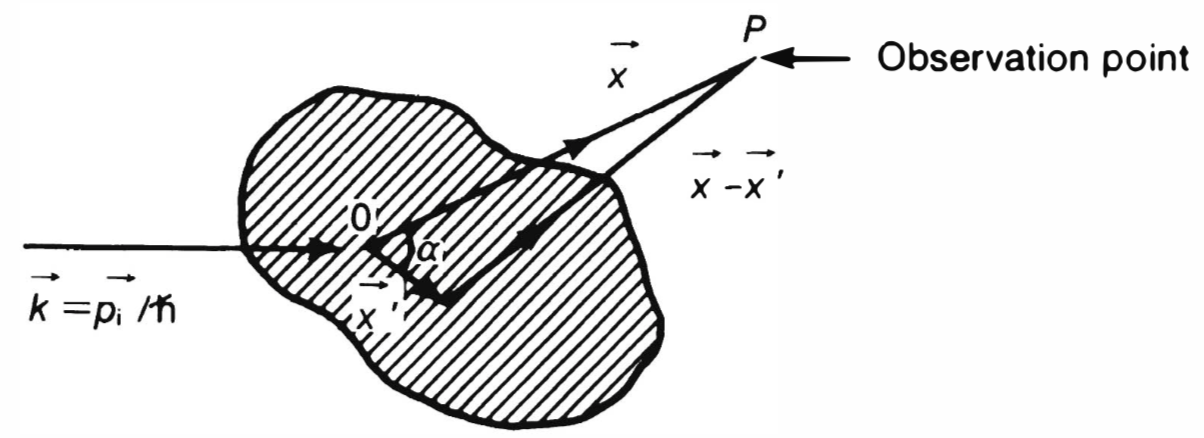
\includegraphics[width=10cm]{Scattering/sourcefields.png}
\caption{我们在场点$x$观察粒子的散射,而散射发生的区域则局限在源点$x'$。}
%\label{default}
\end{center}
\end{figure}

在远场条件下,

\begin{eqnarray*}
|x-x' |  & = & \sqrt{ r^2 + r'^2 - 2 r r' \cos \alpha }  \\ 
{} & = & r \sqrt{ 1- \frac{2r'}{r} \cos \alpha + \frac{r'^2}{r^2 } } \\
{} & \approx & r- \hat r \cdot x'
\end{eqnarray*}

这里

\begin{equation}
\hat r = \frac{x}{|x|}
\end{equation}

出射波函数波矢

\begin{equation}
k' = k \hat r
\end{equation}

这样

\begin{equation}
e^{\pm i k |x-x'| } \approx e^{\pm i k r} e^{\mp i k' \cdot x'}
\end{equation}

这里$k'$表示散射后的波矢,它的方向在空间某个$( \theta, \phi )$的取向上。由于弹性散射,它的大小还是$k$,$k'$的方向与矢径$r$的方向相同,对应$e^{i k r}$。

在远场条件下,出射波函数$\psi^{(+)}$为,

\begin{equation}
\left\langle x | \psi^{(+)}\right\rangle = \left\langle x | k \right\rangle - \frac{1}{4 \pi} \frac{2m}{\hbar^2} \frac{e^{i k r}}{r} \int d^3 x' e^{- i k' \cdot x' } V(x') \left\langle x' | \psi^{(+)}\right\rangle
\label{OutgoingWaveFunction}
\end{equation}

定义

\begin{eqnarray*}
f(k',k) & = & \frac{1}{4 \pi} \frac{2m}{\hbar^2} (2\pi)^3 \int d^3 x' \frac{e^{-i k' \cdot x'}}{(2 \pi)^{3/2}} V(x') \left\langle x' | \psi^{(+)} \right\rangle \\
{} & = & - \frac{1}{4\pi}(2 \pi)^3 \frac{2m}{ \hbar^2 } \left\langle k' \right| V \left| \psi^{(+)} \right\rangle
\end{eqnarray*}

假设入射波在$\hat z$方向上,$\psi^{(+)} (x)$现在可写为:

\begin{equation}
\psi^{(+)} (x) = \frac{1}{(2 \pi)^{3/2}} \left[ e^{i k z} + \frac{e^{ikr}}{r} f(k', k)  \right]
\end{equation}

对上式,我们可分别计算入射几率流$j_i$和散射几率流$j_s$:

\begin{eqnarray}
j_i & = & \frac{\hbar k}{m} \\
j_s & = & \frac{\hbar k}{m} \frac{|f(k', k)|^2}{r^2}
\end{eqnarray}

散射粒子数$dn$

\begin{equation}
d n = j_s r^2 d \Omega
\end{equation}

应正比于入射流$j_i$,立体角微元$d \Omega$和微分散射截面\index{Differential cross-section:微分散射截面}$\sigma_c = \frac{d \sigma}{d \Omega}$。

\begin{equation}
d n = \sigma_c j_i d \Omega
\end{equation}

因此,

\begin{equation}
\sigma_c = \frac{d \sigma}{d \Omega} = \frac{d n}{ j_i d \Omega  }=\frac{ j_s r^2 d \Omega }{j_i d \Omega} = |f(k',k)|^2
\end{equation}

所谓一阶的玻恩近似\index{Born Approximation:玻恩近似}就是直接用$\left| k \right\rangle$代替公式[\ref{OutgoingWaveFunction}]右侧的$\left| \psi^{(+)} \right\rangle$ 。

\subsection{高阶玻恩近似}

把公式[\ref{OutgoingWaveFunction}]右侧的$V \left| \psi^{(+)} \right\rangle$形式地改写为:

\begin{equation}
V \left| \psi^{(+)} \right\rangle = T \left| \phi \right\rangle 
\end{equation}

考虑到李普曼-施温格方程,

\begin{equation}
V \left| \psi^{(+)} \right\rangle = V \left| \phi \right\rangle + V \frac{1}{E- H_0 + i \epsilon} T \left| \phi \right\rangle = T \left| \phi \right\rangle
\end{equation}

这意味着

\begin{equation}
T = V + V \frac{1}{E - H_0 + i \epsilon} T
\end{equation}

散射振幅$f(k',k)$可写为,

\begin{equation}
f(k',k) = - \frac{1}{4 \pi} \frac{2m}{\hbar^2} (2\pi)^3 \left\langle k' \right| T \left| k \right\rangle
\end{equation}

变换矩阵可以一直迭代下去:

\begin{equation}
T = V + V \frac{1}{E - H_0 + i \epsilon} V + V \frac{1}{E - H_0 + i \epsilon} V \frac{1}{E - H_0 + i \epsilon} V + ...
\end{equation}

相互作用$V$出现几次,就是几阶玻恩近似。

\subsection{光学定理}

\begin{equation}
\Im f(\theta = 0) = \frac{k \sigma_t}{4 \pi}
\end{equation}

这里$\theta =0$表示向前散射\index{forward scattering:向前散射}(forward scattering),$k' = k$。$\sigma_t$表示总散射截面(即空间各取向微分散射截面的总和)

\begin{equation}
\sigma_t = \int \frac{d \sigma }{d \Omega} d \Omega
\end{equation}

证明如下,首先:

\begin{equation}
f(\theta = 0) = f(k,k) = - \frac{1}{4 \pi}\frac{2m}{\hbar^2} (2 \pi)^3 \left\langle k \right| T \left| k \right\rangle
\end{equation}

考虑$\left\langle k \right| T \left| k \right\rangle$的虚部。这里:

\begin{equation}
\left| k \right\rangle = \left| \psi^{(+)} \right\rangle - \frac{1}{E - H_0 + i \epsilon} V \left| \psi^{(+)} \right\rangle
\end{equation}

因此:

\begin{eqnarray*}
\Im \left\langle k \right| T \left| k \right\rangle & = & \Im \left\langle k \right| V \left| \psi^{(+)} \right\rangle \\
{} & = & \Im \left[  \left(  \left\langle \psi^{(+)} \right| -  \left\langle \psi^{(+)} \right| V \frac{1}{E - H_0 - i \epsilon} \right) V \left| \psi^{(+)} \right\rangle     \right]
\end{eqnarray*}

上式中第一项是实的,第二项要考虑含有虚数的$\frac{1}{E - H_0 - i \epsilon}$,

\begin{equation}
\frac{1}{E - H_0 - i \epsilon} = P \frac{1}{E- H_0} + i \pi \delta(E - H_0)
\end{equation}

上式第一项贡献是实的,第二项则是纯虚的贡献,

\begin{eqnarray*}
\Im \left\langle k \right| T \left| k \right\rangle & = & - \pi \left\langle \psi^{(+)} \right| V \delta (E - H_0) V \left| \psi^{(+)} \right\rangle \\
{} & = & - \pi \left\langle k \right| T^\dagger \delta (E - H_0) T \left| k \right\rangle \\
{} & = & - \pi \int d^3 k' \left\langle k' \right| T^\dagger \left| k' \right\rangle \left\langle k' \right| T \left| k \right\rangle \delta(E - \frac{\hbar^2 k'^2}{2m})
\end{eqnarray*}

这里

\begin{equation}
d^3 k' = k'^2 dk' d \Omega' = k'^2  \left( \frac{dk'}{dE} \right) dE d \Omega'
\end{equation}

考虑到$E = \frac{\hbar^2 k'^2}{2m}$,$dE = \frac{\hbar^2 k'}{m} dk'$

\begin{equation}
\frac{d k'}{d E } = \frac{m }{\hbar^2 k'}
\end{equation}

$\delta(E - \frac{\hbar^2 k'^2}{2m})$意味着$k' = k$,$d \Omega'$是对立体角的积分,与径向无关。

\begin{equation}
\Im  \left\langle k \right| T \left| k \right\rangle = - \pi \int d \Omega' \frac{mk}{\hbar^2}  | \left\langle  k' | T | k \right\rangle  |^2
\end{equation}

因此:

\begin{equation}
\Im f(0) = \frac{ k \sigma_t}{4 \pi }
\end{equation}

这就是所谓光学定理\index{optical theorem:光学定理}(optical theorem)。证明的过程中需要用到$f(0)$,$f(k',k)$,和$\Im \left\langle k \right| T \left| k \right\rangle $ 的表达式。


\subsection*{参考}

J. J. Sakurai, Modern Quantum Mechanics, \S 7.1, 7.2, 7.3